\documentclass[tikz,border=4pt]{standalone}
\usepackage{amsmath,amssymb}\renewcommand{\familydefault}{\sfdefault}
\usepackage{pgfplots}\pgfplotsset{compat=1.17}
\usetikzlibrary{arrows.meta,positioning,shadows,fit,calc,backgrounds,patterns}
\definecolor{lav}{HTML}{E6E6FF}\definecolor{pinkb}{HTML}{FFDDDD}\definecolor{greenb}{HTML}{DDFFDD}\definecolor{yelb}{HTML}{FFFBCF}\definecolor{peach}{HTML}{FFEBD6}\definecolor{mauve}{HTML}{F0E6F0}
\definecolor{reqblue}{HTML}{0000BB}\definecolor{resgreen}{HTML}{008800}\definecolor{dred}{HTML}{CC0000}\definecolor{domblue}{HTML}{000099}\definecolor{crimson}{HTML}{990033}
\definecolor{tbBlue}{HTML}{1F77B4}\definecolor{tbOrange}{HTML}{FF7F0E}\definecolor{tbGreen}{HTML}{2CA02C}\definecolor{tbRed}{HTML}{D62728}\definecolor{tbPurple}{HTML}{9467BD}\definecolor{tbBrown}{HTML}{8C564B}
\definecolor{barGreen}{HTML}{1B8754}\definecolor{darkGreen}{HTML}{2E7D32}\definecolor{lightBlue}{HTML}{A0C4FF}\definecolor{kRed}{HTML}{DC3545}
\definecolor{accB}{HTML}{3366FF}\definecolor{f1O}{HTML}{FF7F50}\definecolor{aucG}{HTML}{44CC11}
\tikzset{node/.style={draw,rounded corners=2.5pt,thick,align=center},
 req/.style={-{Stealth[length=2.4mm]},thick,reqblue},res/.style={-{Stealth[length=2.4mm]},thick,dashed,resgreen}}
\pgfplotsset{every axis/.append style={tick label style={font=\footnotesize},label style={font=\small},title style={font=\small},legend style={font=\footnotesize,fill=white,fill opacity=.9,text opacity=1,draw=black!25,rounded corners=1pt},
 grid style={dotted,black!35}}}
\begin{document}
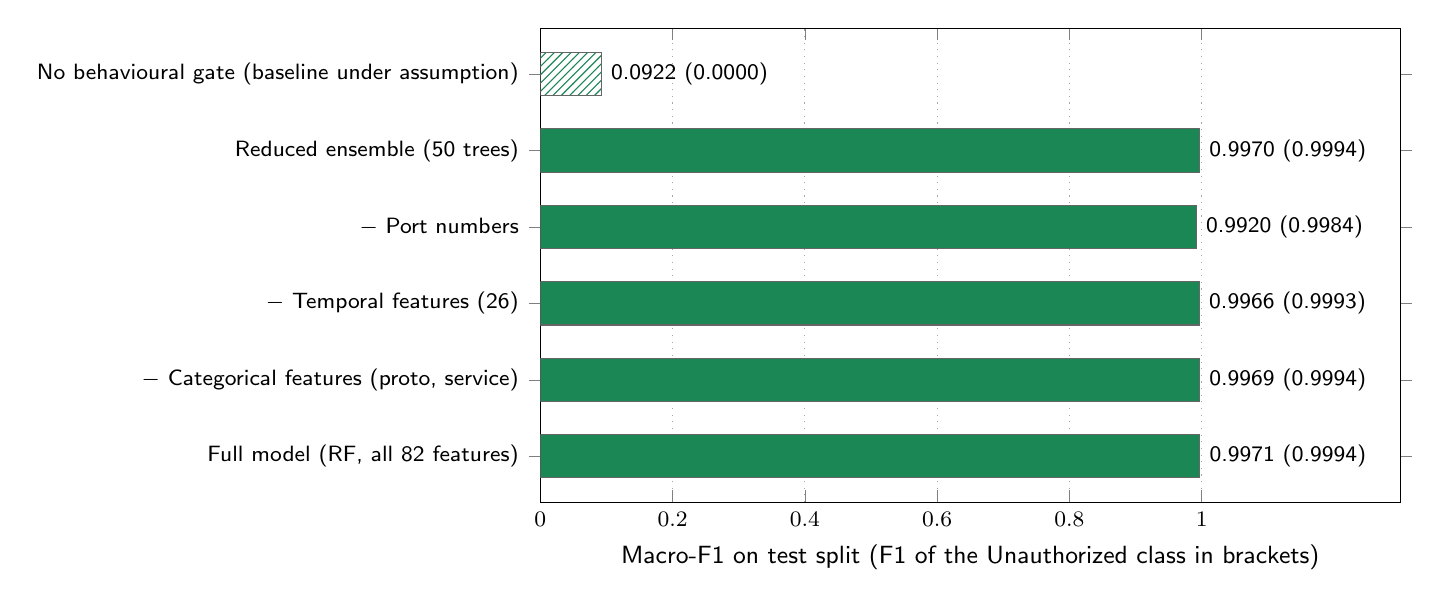
\begin{tikzpicture}\begin{axis}[width=12.5cm,height=7.6cm,xbar,xmin=0,xmax=1.3,ymin=-0.6,ymax=5.6,ytick={0,...,5},yticklabels={{Full model (RF, all 82 features)},{$-$ Categorical features (proto, service)},{$-$ Temporal features (26)},{$-$ Port numbers},{Reduced ensemble (50 trees)},{No behavioural gate (baseline under assumption)}},y tick label style={font=\footnotesize},xlabel={Macro-F1 on test split (F1 of the Unauthorized class in brackets)},xmajorgrids,xtick={0,.2,.4,.6,.8,1}]
\addplot[xbar,bar shift=0pt,fill=barGreen,draw=black!60,bar width=0.55cm,point meta=explicit symbolic,nodes near coords,nodes near coords style={font=\footnotesize,anchor=west}] coordinates {(0.9971,0) [0.9971 (0.9994)]};
\addplot[xbar,bar shift=0pt,fill=barGreen,draw=black!60,bar width=0.55cm,point meta=explicit symbolic,nodes near coords,nodes near coords style={font=\footnotesize,anchor=west}] coordinates {(0.9969,1) [0.9969 (0.9994)]};
\addplot[xbar,bar shift=0pt,fill=barGreen,draw=black!60,bar width=0.55cm,point meta=explicit symbolic,nodes near coords,nodes near coords style={font=\footnotesize,anchor=west}] coordinates {(0.9966,2) [0.9966 (0.9993)]};
\addplot[xbar,bar shift=0pt,fill=barGreen,draw=black!60,bar width=0.55cm,point meta=explicit symbolic,nodes near coords,nodes near coords style={font=\footnotesize,anchor=west}] coordinates {(0.9920,3) [0.9920 (0.9984)]};
\addplot[xbar,bar shift=0pt,fill=barGreen,draw=black!60,bar width=0.55cm,point meta=explicit symbolic,nodes near coords,nodes near coords style={font=\footnotesize,anchor=west}] coordinates {(0.9970,4) [0.9970 (0.9994)]};
\addplot[xbar,bar shift=0pt,pattern=north east lines,pattern color=barGreen,draw=black!60,bar width=0.55cm,point meta=explicit symbolic,nodes near coords,nodes near coords style={font=\footnotesize,anchor=west}] coordinates {(0.0922,5) [0.0922 (0.0000)]};
\end{axis}\end{tikzpicture}
\end{document}
